%--------------------------------------------%
%--------------------------------------------%
%    INTROCUTION 
%--------------------------------------------%
%--------------------------------------------%

\section{Introduction}
%    CLUSTERING
%--------------------------------------------%
\subsection{Clustering}

% FRAME: WHAT IS CLUSTERING
\begin{frame}{What is clustering?}

``The goal of data clustering, also known as cluster analysis, is to discover the natural grouping(s) of a set of patterns, points, or objects.''
\footnote{A. K. Jain, “Data clustering: 50 years beyond K-means,” Pattern Recognition Letters, vol. 31}
%{\scriptsize A. K. Jain, “Data clustering: 50 years beyond K-means,” Pattern Recognition Letters, vol. 31}

\end{frame}
        
% FRAME: DIFFERENT CLUSTERING ALGORITHMS
% \begin{frame}{What is clustering?}

% \centering
% \includegraphics[width=0.8\columnwidth]{{{diff_algs_Fred2005}}}

% {\fontsize{5.5}{5.5} \selectfont Source: A. N. L. Fred and A. K. Jain, “Combining multiple clusterings using evidence accumulation,” IEEE Transactions on Pattern Analysis and Machine Intelligence, vol. 27}

% \end{frame}

\begin{frame}{What is clustering?}
\centering
\begin{tabular}{ccc}
  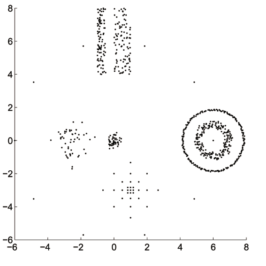
\includegraphics[width=0.3\textwidth]{diff_algs/raw} &   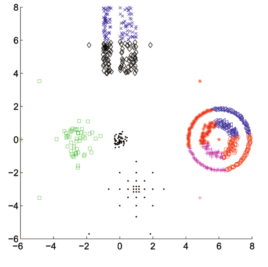
\includegraphics[width=0.3\textwidth]{diff_algs/b} & 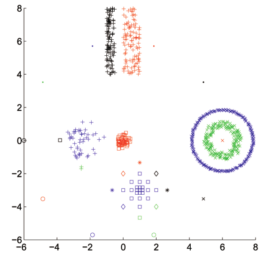
\includegraphics[width=0.3\textwidth]{diff_algs/c}  \\

  {\tiny (a)} & {\tiny (b)} & {\tiny (c)} \\

  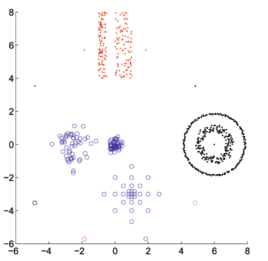
\includegraphics[width=0.3\textwidth]{diff_algs/d} &  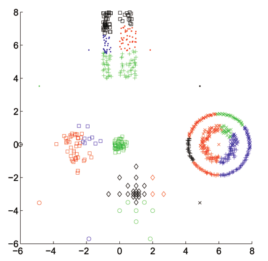
\includegraphics[width=0.3\textwidth]{diff_algs/e} &  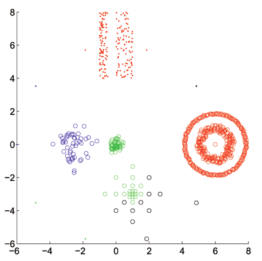
\includegraphics[width=0.3\textwidth]{diff_algs/f}\\

  {\tiny (d)} & {\tiny (e)} & {\tiny (f)}

\end{tabular}
{\fontsize{5.5}{5.5} \selectfont A. N. L. Fred and A. K. Jain, “Combining multiple clusterings using evidence accumulation”, IEEE Transactions on Pattern Analysis and Machine Intelligence, vol. 27}

\end{frame}


%--------------------------------------------%
%    EAC
%--------------------------------------------%
\subsection{EAC}
\begin{frame}{Evidence Accumulation Clustering}

\begin{itemize}
	\item State-of-the-art

	\item Robust

	\item Ensemble method

	% \item Robust state-of-the-art ensemble method

	% \item Three steps:
	% \begin{itemize}
	% 	\item \textbf{Production} of a clustering ensemble
	% 	\item \textbf{Combination} into a co-association matrix
	% 	\item \textbf{Recovery} of the natural clusters
	% \end{itemize}

	% \item More complex and computationally expensive

	% \item Harder to scale

\end{itemize}

\end{frame} 

\begin{frame}{EAC: Production}

\centering
\begin{tabular}{ccc}
  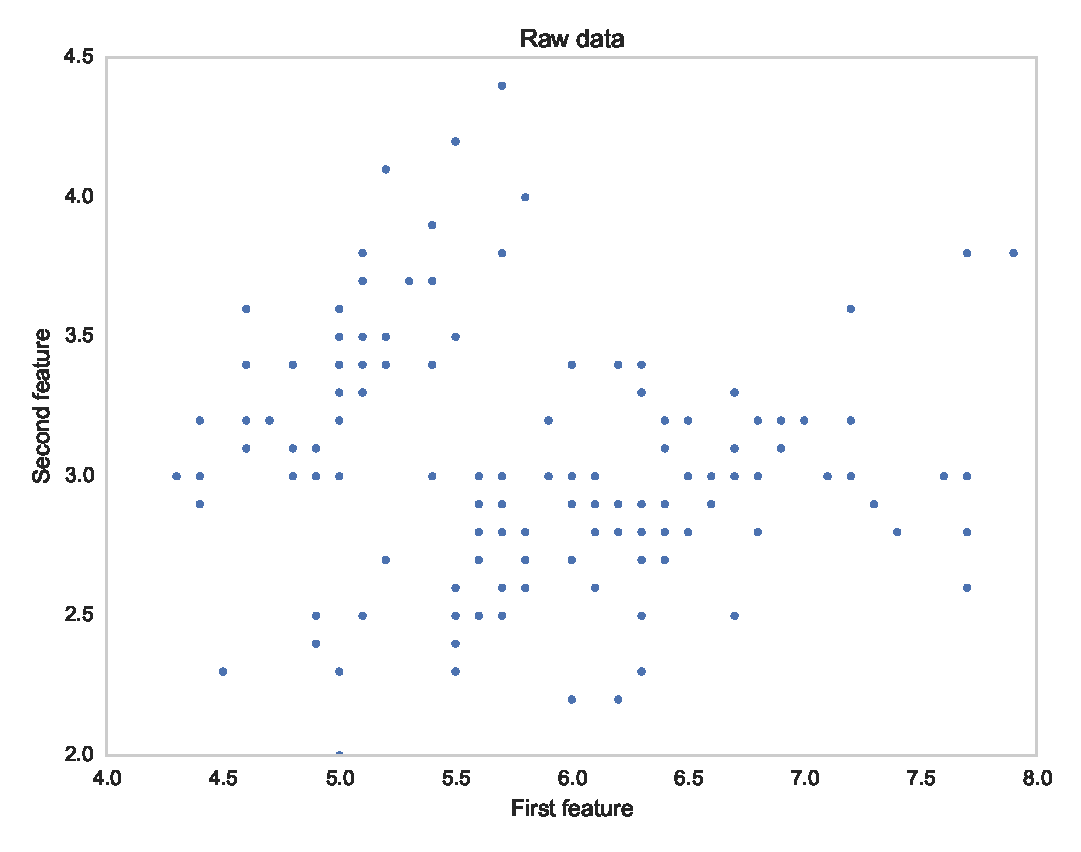
\includegraphics[width=0.3\textwidth]{EAC_plots/raw_data} &  & 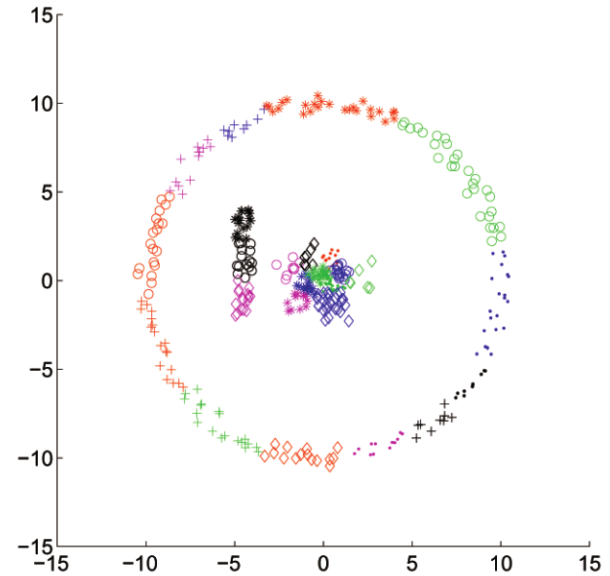
\includegraphics[width=0.3\textwidth]{EAC_plots/kmeans1} \\
 
   {\tiny (a)} & & {\tiny (b)} \\

  & &  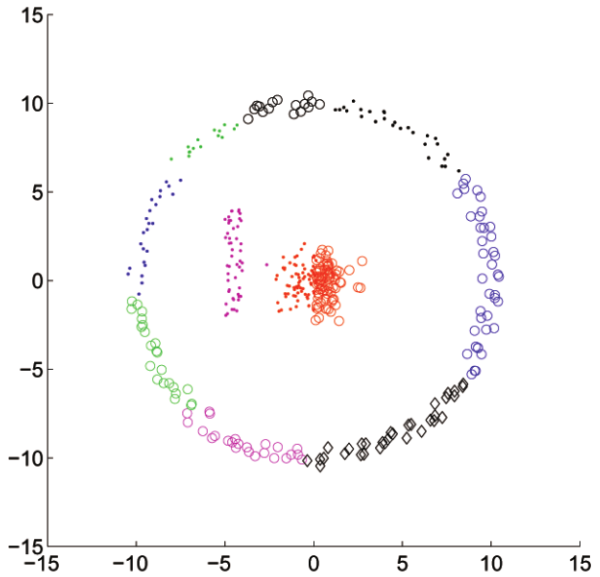
\includegraphics[width=0.3\textwidth]{EAC_plots/kmeans2} \\

  & & {\tiny (c)} \\
\end{tabular}

% {\fontsize{5.5}{5.5} \selectfont Source: A. N. L. Fred and A. K. Jain, “Combining multiple clusterings using evidence accumulation,” IEEE Transactions on Pattern Analysis and Machine Intelligence, vol. 27}

\end{frame}




\begin{frame}{EAC: Combination}

\centering
\begin{tabular}{ccc}
  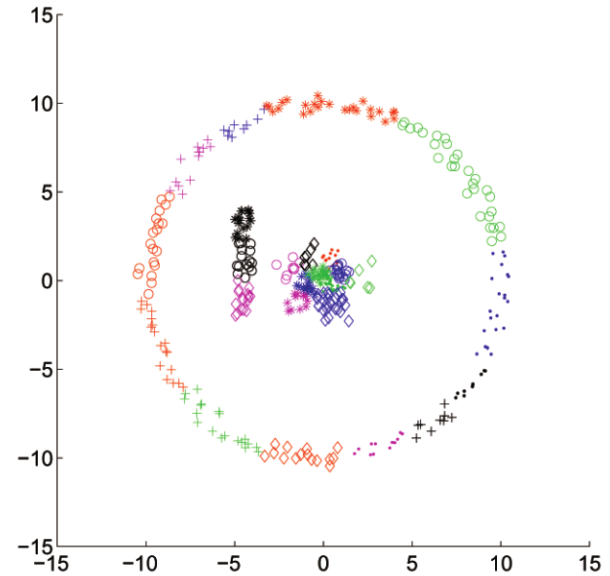
\includegraphics[width=0.3\textwidth]{EAC_plots/kmeans1} &   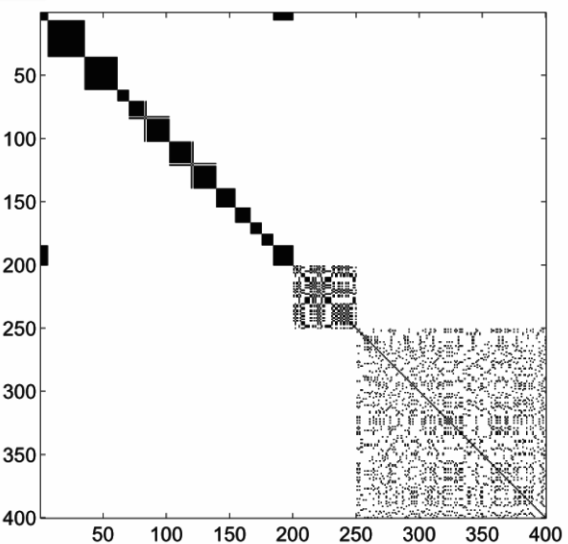
\includegraphics[width=0.3\textwidth]{EAC_plots/coassoc1} & 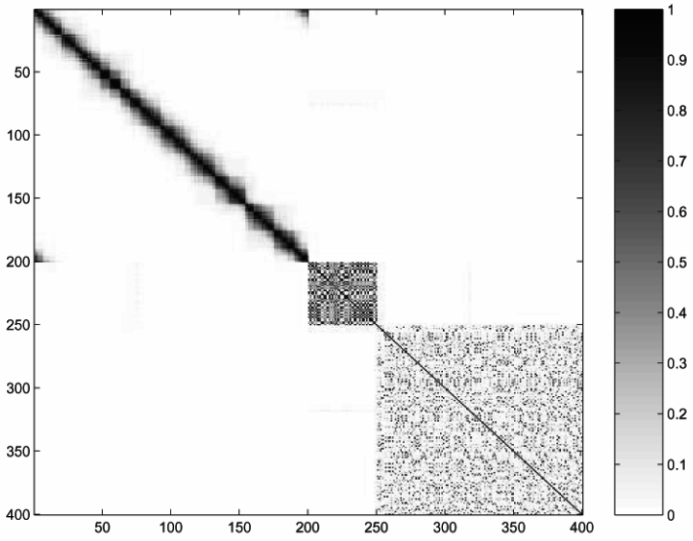
\includegraphics[width=0.3\textwidth]{EAC_plots/coassocEAC}  \\

  {\tiny (a)} & {\tiny (c)} & {\tiny (e)} \\

  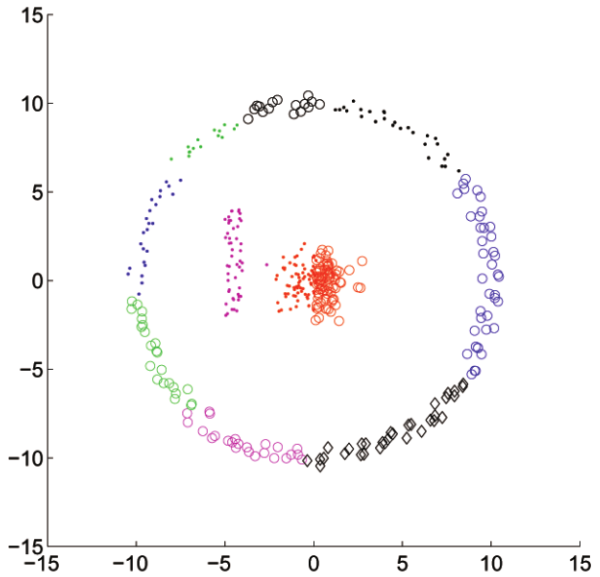
\includegraphics[width=0.3\textwidth]{EAC_plots/kmeans2} &  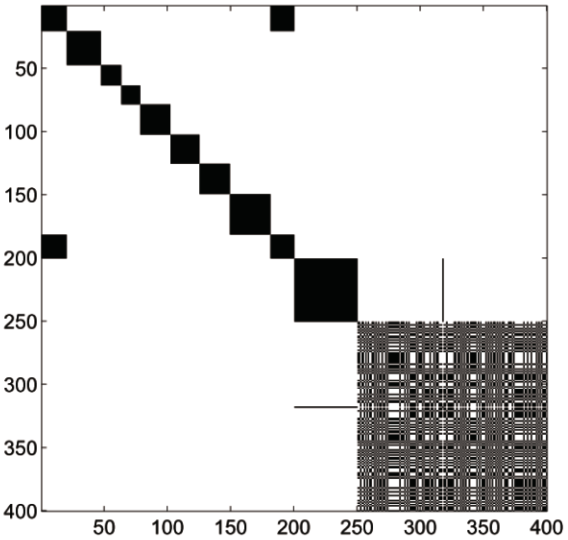
\includegraphics[width=0.3\textwidth]{EAC_plots/coassoc2} & \\

  {\tiny (b)} & {\tiny (d)} &

\end{tabular}

% {\fontsize{5.5}{5.5} \selectfont Source: A. N. L. Fred and A. K. Jain, “Combining multiple clusterings using evidence accumulation,” IEEE Transactions on Pattern Analysis and Machine Intelligence, vol. 27}

\end{frame}

\begin{frame}{EAC: Recovery}

\centering
\begin{tabular}{cc}
  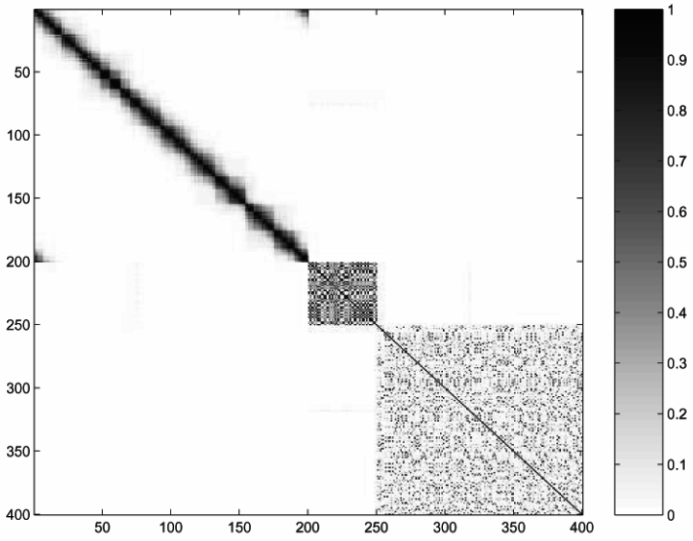
\includegraphics[width=0.3\textwidth]{EAC_plots/coassocEAC} &   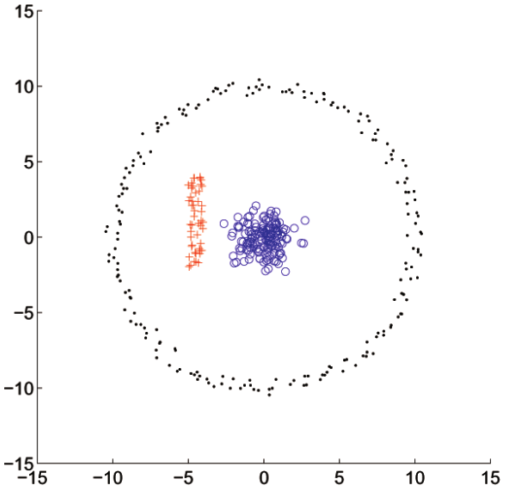
\includegraphics[width=0.3\textwidth]{EAC_plots/eac}  \\

  {\tiny (a)} & {\tiny (b)}
\end{tabular}


% {\fontsize{5.5}{5.5} \selectfont Source: A. N. L. Fred and A. K. Jain, “Combining multiple clusterings using evidence accumulation,” IEEE Transactions on Pattern Analysis and Machine Intelligence, vol. 27}

\end{frame}

\subsection{Goals}

\begin{frame}{Goals}
\begin{itemize}
% \item Study the integration of quantum inspired methods in EAC.
% \item Study the integration of the GPGPU paradigm in EAC.
\item Devise strategies to reduce computation and memory complexities of EAC.
\item Validation of Big Data EAC on real data.
\item Application of Evidence Accumulation Clustering to Big Data.
%\item Application of EAC to real-world large datasets.
\end{itemize}
\end{frame}    	